% CVPR 2026 camera-ready format
% Machine Learning Assignment 2 -- Kumar Gaurav -- P26AI0006
\documentclass[10pt,twocolumn,letterpaper]{article}

\usepackage{cvpr}
\usepackage{amsmath,amssymb}
\usepackage{booktabs}
\usepackage{graphicx}
\usepackage{xcolor}
\usepackage{url}
\usepackage[breaklinks,colorlinks,allcolors=cvprblue]{hyperref}

\definecolor{cvprblue}{rgb}{0.21,0.49,0.74}

% Tighten float spacing so the eight-page body can hold all required evidence.
\setlength{\textfloatsep}{6pt plus 2pt minus 2pt}
\setlength{\floatsep}{5pt plus 2pt minus 2pt}
\setlength{\intextsep}{5pt plus 2pt minus 2pt}
\setlength{\abovecaptionskip}{3pt}
\setlength{\belowcaptionskip}{0pt}

\input{generated/numbers.tex}

\title{When Bagging Beats Boosting:\\
Single Trees, Bootstrap Aggregation, and SAMME\\ on Raw Olivetti Faces}

\author{Kumar Gaurav\\
Roll No. P26AI0006\\
Machine Learning Assignment 2\\
\small Repository: \url{\RepoURL}\\
\small Commit: \texttt{\CommitHash}}

\begin{document}
\maketitle

\begin{abstract}
We study closed-set face identification from raw $64\times64$ Olivetti images
under a frozen, roll-number-seeded split of six training, two validation and two
test images per identity.  We compare a single CART tree, bootstrap aggregation
(bagging) with up to 200 trees, and a from-scratch SAMME multiclass AdaBoost.
Every choice is made on clean validation accuracy; a centred $16\times16$ block
is zeroed only at test time.  The selected single tree overfits (training
accuracy 1.0000, 41 leaves) and reaches 0.6000 validation and 0.5000 test
accuracy.  Bagging with $B=200$ reaches 0.9250 validation and 0.8375 clean test
accuracy, and retains 0.7375 when the central block is zeroed.  SAMME with depth
4 and 50 rounds reaches 0.4375 validation and 0.3875 test accuracy, and 0.2750
masked.  Thirty within-identity bootstrap resamples show that bagging cuts measured
variance by a factor of \BagVarRatio, while squared bias rises from
\TreeFinalBias~to \BagFinalBias; the variance reduction dominates and refit
accuracy improves from \TreeRefitAcc~to \BagRefitAcc.  We report the unsuccessful
and ambiguous outcomes as well: boosting's hard-vote multiclass decisions remain
weak on 240 training faces, and in a masked case where bagging still gives the
true identity 49 of 200 votes, boosting's normalised score for that identity is
only 0.1484.
\end{abstract}

\section{Introduction}

Face identification from raw pixels is a deliberately unfriendly test bed for
classical classifiers.  Each image is a 4096-dimensional vector, only 240
images are available for training, and the forty identities are separated by
subtle lighting, pose and expression changes.  A decision tree can fit this
training set perfectly by isolating individual faces, but such a tree has no
reason to generalise.  Ensembling is the natural response: bagging attacks
variance by averaging trees fitted to bootstrap resamples, while boosting
attacks bias by reweighting examples that the current weak learners get wrong.

This report answers the three questions of Machine Learning Assignment 2 under
one fixed protocol.  The split is generated once from the seed obtained by
reading every numeric character of the roll number \texttt{P26AI0006} in order,
namely $\Seed$, and is reused by every experiment.  The split assigns six
training, two validation and two test images to each of the forty identities.
Model selection uses clean validation accuracy only.  The clean test set is
touched only for the final reporting requested by the assignment, and the masked
test set is never used for training or selection.  No PCA or other
dimensionality reduction is applied.

Our contributions are: (i) an exact, saved split and a complete Q1--Q3
pipeline with deterministic seeds and artifact checks; (ii) student
implementations of bagging and SAMME, including explicit rejection of weak
learners that are no better than random; (iii) a diagnostic study of out-of-bag
error, pairwise disagreement, vote margins, sample-weight concentration and
masked-test behaviour; and (iv) a measured bias--variance decomposition over 30
within-identity bootstrap resamples.  The headline is that bagging is the clear
winner here, while SAMME is stable but weak: its weighted training error falls
from 0.8500 to 0.6143, yet its hard-vote accuracy on the test set is 0.3875,
below the single tree's 0.5000.

\section{Protocol and Reproducibility}

\subsection{Data and frozen split}

We use \texttt{sklearn.datasets.fetch\_olivetti\_faces}~\cite{samaria1994}: 40
identities, ten images each, $64\times64$ pixels, values in $[0,1]$.  The compact cache is
stored as \texttt{data/olivetti\_faces.npz}; its image array hashes to
\texttt{\DataHash}.  The seed rule gives
\begin{equation}
\text{seed} = \text{all digits of \texttt{P26AI0006} in order} = \Seed.
\end{equation}
A single \texttt{numpy.random.default\_rng(260006)} stream is consumed identity
by identity in ascending order.  For each identity the ten dataset indices are
permuted once; the first six become training images, the next two validation
images and the last two test images.  The resulting 240/80/80 partition has
SHA-256 \texttt{\SplitHash} and is saved to \texttt{results/split.npz} and
\texttt{results/split.csv}.  Every script loads this file; the split is never
regenerated inside an experiment.

\subsection{Masked test set and selection discipline}

For the masked condition we copy the test matrix and set rows 24--39 and
columns 24--39 of every image to zero, i.e.\ a centred $16\times16$ block.  All
other pixels are unchanged.  Training and validation images remain clean.  The
mask is applied only when evaluating a fitted model.  This is a response test,
not a training augmentation.

Every hyperparameter and every ensemble size is selected by clean validation
accuracy.  Ties are resolved by the first row in a fixed grid order (shallower
depth, then smaller leaf, then smaller $B$ or fewer rounds).  The clean test
column is reported after selection; it is not used to choose a model.  The
masked test column is reported for the selected models and for the bagging
$B$-grid, but never enters a selection rule.

\subsection{Implementation}

\texttt{scikit-learn}'s~\cite{pedregosa2011}
\texttt{DecisionTreeClassifier} is the only base
learner, as permitted by the assignment.  Bagging and SAMME are implemented in
\texttt{src/common.py}.  The bagging implementation draws one nested sequence of
200 bootstrap replicates and 200 tree seeds; an ensemble of size $B$ is exactly
the first $B$ trees of the 200-tree ensemble.  This makes the $B$-curve paired
rather than a collection of independently seeded runs.  SAMME fits each tree
with the current sample weights, records the weighted error, $\alpha_t$ and the
weight distribution, and stops explicitly if a learner is no better than
random.  The full pipeline is \texttt{python -m src.run\_all}; the run log, the
resolved configuration, a pip freeze and SHA-256 manifests of every result file
are stored under \texttt{results/}.  The complete run took
\RuntimeHours~hours on the run machine.

\section{Q1: Single Trees and Bagging}

\subsection{Decision-tree grid}

The grid crosses maximum depth $\{2,4,8,16,\text{unrestricted}\}$ with minimum
leaf size $\{1,2,4\}$, giving fifteen trees.  Figure~\ref{fig:tree} plots
validation accuracy and the selected leaf size.  Accuracy rises monotonically
with depth; shallow trees underfit badly (depth 2 reaches 0.0750 validation
accuracy, depth 16 reaches 0.2875), and the unrestricted tree is the only one
that crosses 0.5.  The selected configuration is unrestricted depth with
\texttt{min\_samples\_leaf}$=1$: training 1.0000, validation 0.6000, test
0.5000.  It has \TreeLeaves~leaves, \TreeMeanLeaf~training samples per leaf on
average, and a singleton-leaf fraction of \TreeSingleton.  Training accuracy of
1.0000 with only 240 samples is the signature of memorisation, not a model of
faces.  The complete grid is in \texttt{results/tree\_grid.csv}.

\begin{figure*}[t]
\centering
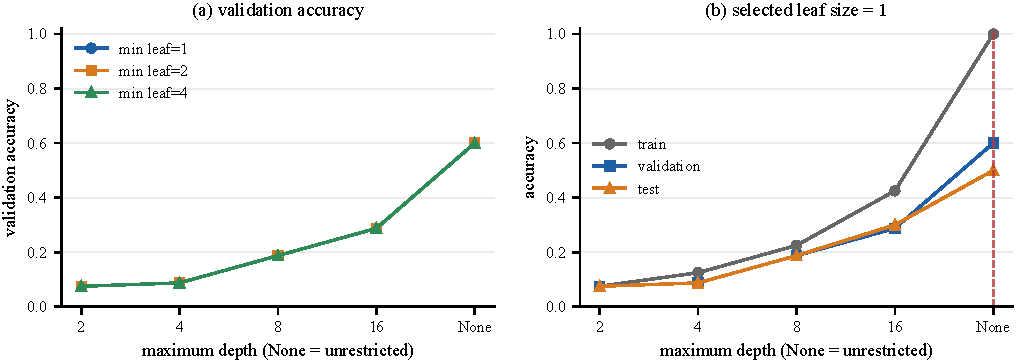
\includegraphics[width=0.86\linewidth]{../figures/fig1_tree_grid.pdf}
\caption{Q1 tree grid.  (a) Validation accuracy for the fifteen
depth $\times$ leaf-size combinations; unrestricted depth is the only setting
above 0.5.  (b) Train, validation and test accuracy at the selected leaf size
1.  The dashed line marks the selected unrestricted tree.  Training accuracy
reaches 1.0000 while validation stalls at 0.6000.}
\label{fig:tree}
\end{figure*}

\subsection{Bagging and the ensemble-size curve}

Bagging~\cite{breiman1996,breiman2001} fits $B$ trees to bootstrap resamples of
the 240 training images and predicts by plurality vote.  Table~\ref{tab:bagging} and
Figure~\ref{fig:bagging} report $B\in\{1,5,10,25,50,100,200\}$.  A single
bootstrap tree ($B=1$) reaches 0.4625 validation and 0.3875 test accuracy,
which is worse than the tree fitted to all training data; one bootstrap sample
is a poor classifier.  Averaging fixes this quickly: $B=10$ gives 0.7625
validation, $B=50$ gives 0.8500, and $B=200$ gives 0.9250 validation and
0.8375 test accuracy.  Training accuracy is already 1.0000 at $B=10$; every
additional tree reduces variance rather than training error.  $B=200$ is
selected because it has the highest validation accuracy; $B=100$ is close
(0.9000 validation) and reaches the same 0.8375 test accuracy.

\input{generated/tables/bagging.tex}

\begin{figure*}[t]
\centering
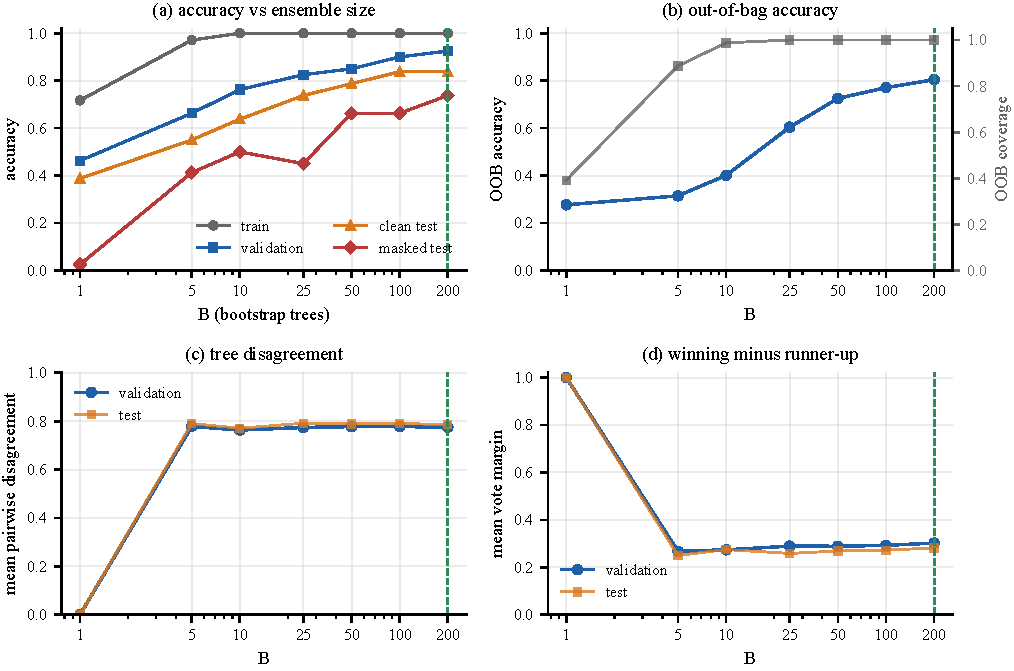
\includegraphics[width=0.86\linewidth]{../figures/fig2_bagging.pdf}
\caption{Bagging diagnostics.  (a) Accuracy versus $B$ on train, clean
validation, clean test and masked test.  (b) Out-of-bag accuracy and coverage.
(c) Mean pairwise disagreement between tree predictions.  (d) Mean winning
minus runner-up vote margin.  The dashed line marks the selected $B=200$.}
\label{fig:bagging}
\end{figure*}

\subsection{Out-of-bag error, disagreement and margin}

Out-of-bag accuracy at $B=200$ is \BagOOB, close to the 0.8375 test estimate and
well above the single tree's 0.5000.  Coverage is 1.0: every training image is
out of bag for at least one of the 200 trees, so the OOB estimate uses all 240
training images rather than a shrinking subset.  The mean number of distinct
training indices per bootstrap sample is \BagDistinct, against the theoretical
\BagDistinctTheory; the implementation therefore draws the intended
with-replacement samples.

Trees disagree on \BagDis~of validation pairs on average.  This is healthy
diversity, not noise: if every tree made the same error, averaging could not
help.  The mean winning-minus-runner-up vote margin is \BagMargin.  A margin of
roughly 0.30 means the winning identity holds about 30 percentage points more
votes than the second identity, which is a useful confidence signal.  The
relationship is not monotone in $B$ (the margin moves from 0.2675 at $B=5$ to
0.3023 at $B=200$) because adding trees can move both the winner and the
runner-up.  The three diagnostics do not tell one story: OOB accuracy and vote
margin improve with $B$, while pairwise disagreement jumps to about 0.78 by
$B=5$ and then stays almost flat.  Disagreement measures diversity, not
correctness; OOB accuracy and margin are the quantities that track accuracy.

\subsection{Clean versus masked test, and face cases}

The masked column of Table~\ref{tab:bagging} is the most striking Q1 result.  A
single bootstrap tree falls to 0.0250 masked accuracy: it has learned splits on
the central pixels and has no redundancy when those pixels are removed.  Five
trees already recover 0.4125; 200 trees reach 0.7375, only 0.1000 below their
clean accuracy.  Averaging many trees makes the prediction robust to the
destruction of one local region even though the individual trees are not
region-invariant.

The confidence numbers reinforce the difference.  On clean images the selected
tree's mean winning confidence is \TreeCleanConf~and bagging's is
\BagCleanConf; under the mask they are \TreeMaskConf~and \BagMaskConf.  The tree
is maximally confident in both conditions, including when it is wrong, while
bagging's confidence falls with its accuracy.  Vote fractions are not calibrated
probabilities, but they are at least sensitive to the loss of evidence.

Figure~\ref{fig:q1cases} shows two faces where bagging corrects the tree and
two where both fail.  In the first correction (dataset index 376, true identity
37) the tree predicts identity 3 with probability 1.0; bagging gives identity
37 \CaseOneVotes~of 200 votes, a margin of \CaseOneMargin.  In the second
(dataset index 175, true identity 17) the tree predicts 22; bagging gives
identity 17 \CaseTwoVotes~votes, margin \CaseTwoMargin.  The two shared errors
are more interesting.  For dataset index 2 (true identity 0) the tree predicts
26 and bagging predicts 15 with \CaseThreeVotes~votes, margin \CaseThreeMargin;
for dataset index 154 (true identity 15) both predict 5, bagging with
\CaseFourVotes~votes and margin \CaseFourMargin.  Bagging corrects 28 of the 40
test faces that the tree gets wrong; on the remaining 12 faces both models fail.
The shared errors are confident and visually plausible confusions, not
tie-breaking noise.  This is the boundary of what bagging can fix: it reduces
variance-driven errors on faces that individual trees place on the wrong side of
an unstable split, but it cannot fix systematic confusions where two identities
share appearance features and all bootstrap trees agree.

\begin{figure*}[t]
\centering
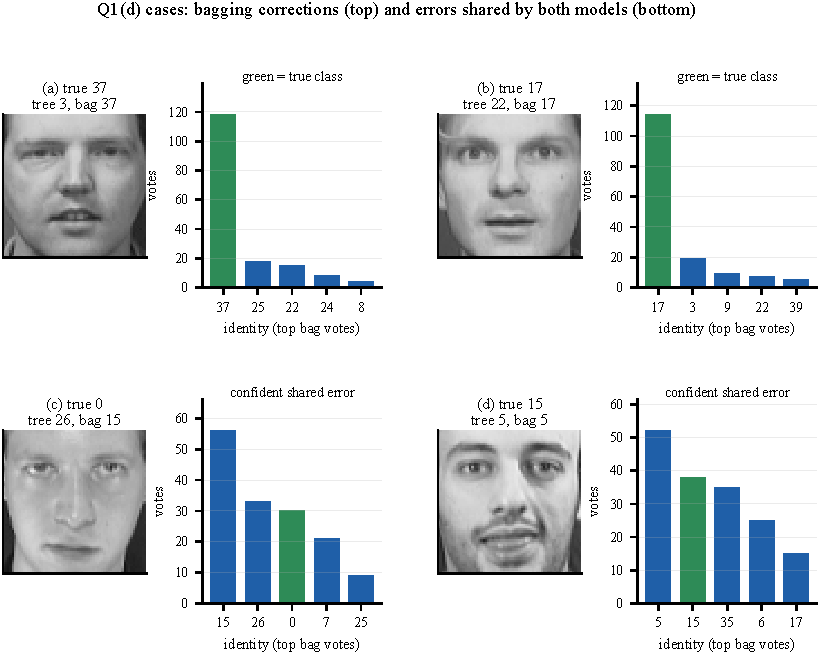
\includegraphics[width=0.86\linewidth]{../figures/fig3_q1_cases.pdf}
\caption{Q1 case studies.  Top row: faces where bagging corrects the single
tree (dataset indices 376 and 175).  Bottom row: faces where both models fail
(indices 2 and 154).  Bars show the five largest bag vote counts; the true
identity is green when it appears in the top five.}
\label{fig:q1cases}
\end{figure*}

\section{Q2: SAMME Boosting}

\subsection{Algorithm and numerical safeguards}

SAMME~\cite{zhu2009,freund1997} is multiclass AdaBoost with hard-label weak
learners.  With $K=40$
classes and training weights $w_i^{(1)}=1/n$, round $t$ fits a tree $h_t$ on the
weighted training set, computes
\begin{equation}
\epsilon_t=\sum_{i=1}^{n} w_i^{(t)}\mathbf{1}[h_t(x_i)\neq y_i],
\end{equation}
and, if $\epsilon_t<1-1/K$, assigns
\begin{equation}
\alpha_t=\log\frac{1-\epsilon_t}{\epsilon_t}+\log(K-1).
\label{eq:alpha}
\end{equation}
Weights are updated by
\begin{equation}
w_i^{(t+1)}=\frac{w_i^{(t)}\exp\!\left(\alpha_t\mathbf{1}[h_t(x_i)\neq y_i]\right)}
{\sum_{j=1}^{n}w_j^{(t)}\exp\!\left(\alpha_t\mathbf{1}[h_t(x_j)\neq y_j]\right)}.
\label{eq:update}
\end{equation}
The ensemble score for class $k$ is
$S_k(x)=\sum_{t=1}^{T}\alpha_t\mathbf{1}[h_t(x)=k]$, and the normalised
response is
\begin{equation}
q_k(x)=\frac{S_k(x)}{\sum_{t=1}^{T}\alpha_t},\qquad \sum_{k=1}^{K}q_k(x)=1.
\label{eq:q}
\end{equation}
The prediction is $\arg\max_k q_k(x)$.

Two edge cases are handled explicitly.  First, if $\epsilon_t\ge 1-1/K$, the
learner is no better than random and $\alpha_t\le 0$; we reject that round,
record the reason in \texttt{stop\_reason}, and stop rather than assign a
meaningless negative or zero weight.  Second, if $\epsilon_t\le\varepsilon$
with $\varepsilon=10^{-12}$, we clip the error to $\varepsilon$ so that
$\alpha_t$ is finite.  In this run no round was rejected: every requested round
produced a learner with $\epsilon_t<0.975$.

\subsection{One complete toy round}

Table~\ref{tab:toy} works through a three-class, nine-sample, one-dimensional
problem with three samples per class and a depth-1 stump.  The stump predicts
class 1 for the three class-2 samples, so the weighted error is
$\epsilon_1=3/9=1/3$ and
$\alpha_1=\log(2)+\log(2)=1.3863$.  The six correct samples are multiplied by
$e^0=1$ and the three wrong samples by $e^{\alpha_1}=4$; after normalisation the
correct weights are $1/18=0.0556$ and the wrong weights are $2/9=0.2222$.  The
updated weights sum to 1.0000.  This is exactly the behaviour required by
Eqs.~\eqref{eq:alpha}--\eqref{eq:update}: the hard class-2 samples receive four
times the weight of the easy samples before normalisation.

\input{generated/tables/toy.tex}

\subsection{Depth $\times$ rounds grid}

Table~\ref{tab:boostgrid} summarises the 16-run grid
(depths 1--4, requested rounds 10, 25, 50 and 100).  All 16 runs accepted every
requested round.  Depth 1 is too weak: at 100 rounds validation accuracy is only
0.1000.  Depth 4 is clearly better, peaking at 50 rounds with 0.4375 validation
and 0.3875 test accuracy.  More rounds are not monotonically better: 100 rounds
at depth 4 gives 0.4250 validation, slightly below 50 rounds, while training
accuracy is 0.9708 at 50 rounds and the last weighted error is 0.6143.  The
selected model is therefore depth 4, 50 rounds, not the largest grid cell.  Its
last $\alpha_t$ is \BoostAlphaLast, and the 100-round run's final weighted error
(0.6694) is higher than the 50-round run's, so additional rounds are fitting
hard faces rather than improving the ensemble.

\input{generated/tables/boosting_grid.tex}

\subsection{Twenty-five, fifty and one hundred learners}

Table~\ref{tab:boostvsbag} compares bagging and boosting at the three requested
ensemble sizes with the frozen settings.  Bagging is better at every size:
0.7375, 0.7875 and 0.8375 test accuracy at 25, 50 and 100 trees, versus 0.2875,
0.3875 and 0.3750 for SAMME.  Bagging also trains faster in serial-equivalent
time at 25 and 50 learners; at 100 learners the gap narrows because each
boosting round refits a depth-4 tree on reweighted data.  The comparison is
controlled: both families see the same 240 training images, the same clean
validation set and the same test set, and the bagging column uses the same
nested bootstrap sequence as Table~\ref{tab:bagging}.  The bagging times in the
table are sums of per-tree fit times, not wall-clock times distorted by
parallel scheduling.

\input{generated/tables/boost_vs_bag.tex}

\subsection{The face that receives the largest weight}

Figure~\ref{fig:weight} follows dataset index 79 (identity 7), the training face
with the largest final SAMME weight.  Its final weight is \WeightFinal, against
a uniform weight of \WeightUniform---about twenty-one times larger.  It is
misclassified by \WeightNMiss~of the \WeightRounds~weak learners, yet the
cumulative ensemble predicts it correctly from round
\WeightFirstCorrect.  This apparent paradox is the point of boosting: the face
is hard for individual depth-4 trees, so its weight grows, but the ensemble's
accumulated votes are already correct and become more so as later learners
specialise on it.  Figure~\ref{fig:weight}(b) shows the mechanism: a correct
round reduces the weight sharply, but the next tree usually errs again, so the
weight climbs back, and the cycle repeats.  The top ten training faces hold
0.4481 of the total weight, so reweighting is concentrated rather than uniform.

\begin{figure*}[t]
\centering
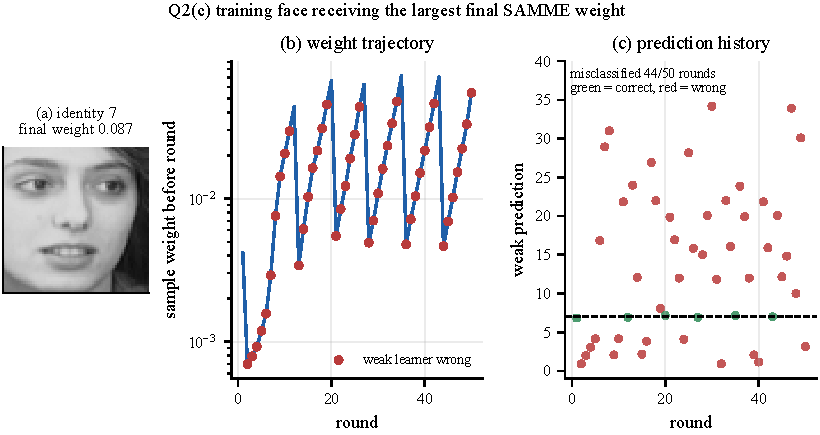
\includegraphics[width=0.86\linewidth]{../figures/fig5_weight_case.pdf}
\caption{The training face with the largest final SAMME weight (dataset index
79, identity 7).  (a) The face and its final weight.  (b) Weight before each
round on a log scale; red points are rounds where the weak learner is wrong.
(c) Weak-learner prediction by round, with the true identity as a dashed line.}
\label{fig:weight}
\end{figure*}

\subsection{Masked response}

Figure~\ref{fig:mask} studies dataset index 170 (true identity 17), a test face
that all three clean models classify correctly.  The full clean and masked
accuracies and mean winning confidences for the three frozen models are in
Table~\ref{tab:final}; here we focus on the face where the two ensembles
diverge.  After masking, the single tree
predicts 13, bagging predicts 17 with \MaskBagTrueVotes~of 200 votes and margin
\MaskBagMargin, and boosting predicts 3.  Boosting's normalised score for the
true identity is only \MaskBoostTrueQ, while its score for identity 3 is
0.1807; the margin between the top two classes is \MaskBoostMargin.  Bagging's
tree disagreement rises from 0.7613 clean to \MaskBagDis~masked, so the
ensemble is genuinely uncertain, but the true class still has a 49-vote lead
over the runner-up.  The mask removes the central 256 pixels, which is where
many identity-specific contours live; bagging survives because its trees make
different errors, while boosting's weighted vote is dominated by learners that
have overfitted to the clean central region.  Boosting's response is also shaped
by its reweighted training distribution: the ten heaviest training faces carry
0.4481 of the sample weight and the single heaviest face (index 79) carries
0.0872, so later learners specialise on a handful of clean central features.
When that region is removed, the $\alpha$-weighted vote has no fallback, whereas
bagging's unweighted plurality still has 49 trees on the true identity.

\begin{figure*}[t]
\centering
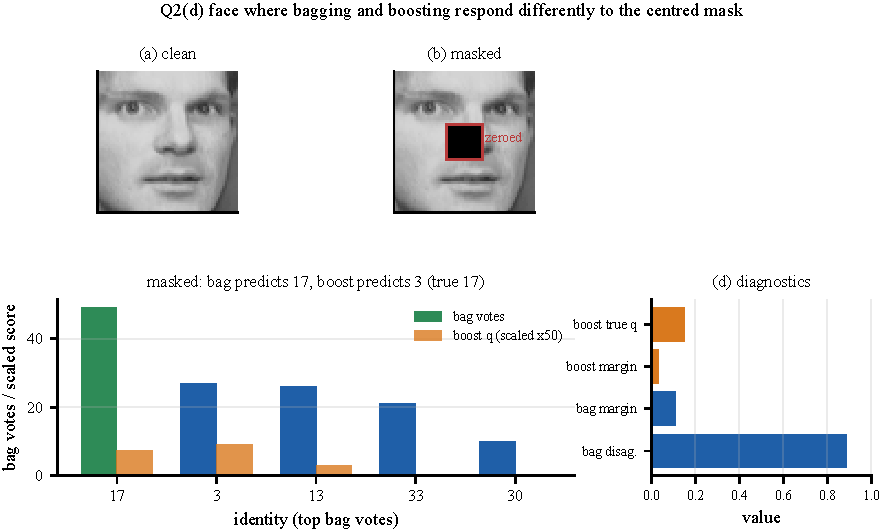
\includegraphics[width=0.86\linewidth]{../figures/fig6_mask_case.pdf}
\caption{Masked-response case (dataset index 170, true identity 17).  (a) Clean
image.  (b) Image with the centred $16\times16$ block zeroed.  (c) Bag votes and
scaled boosting scores for the top five identities.  (d) Disagreement and
margin diagnostics.  Bagging still predicts 17; boosting predicts 3.}
\label{fig:mask}
\end{figure*}

\section{Q3: Measured Bias and Variance}

\subsection{Estimator and resampling design}

For a fixed test image $x_i$ with one-hot target $e_i$, let $p_r(x_i)$ be the
probability vector produced by refit $r$ and let
$\bar p(x_i)=\frac{1}{R}\sum_{r=1}^{R}p_r(x_i)$.  We measure
\begin{equation}
\mathrm{Bias}^2=\frac{1}{N}\sum_{i=1}^{N}\lVert \bar p(x_i)-e_i\rVert_2^2,
\end{equation}
\begin{equation}
\mathrm{Var}=\frac{1}{NR}\sum_{i=1}^{N}\sum_{r=1}^{R}
\lVert p_r(x_i)-\bar p(x_i)\rVert_2^2.
\label{eq:var}
\end{equation}
This is the assignment's Euclidean probability decomposition~\cite{hastie2009},
not the zero-one loss decomposition~\cite{kohavi1996,domingos2000}; the two need
not agree, and accuracy is reported separately.

We draw $R=30$ within-identity bootstrap training sets.  For each identity we
sample six of its six training images with replacement, so every resample has
240 images and the same 6/2/2 identity structure as the original split.  The
selected tree, the 200-tree bag and the selected SAMME model (depth 4, 50
rounds) are refitted from scratch on each resample and evaluated on the same 80
clean test images.  The resample indices are saved in
\texttt{results/q3\_resamples.npz}, and the per-refit probability arrays are
saved in \texttt{results/q3\_predictions.npz}.

\subsection{Selected models}

Table~\ref{tab:final} and Figure~\ref{fig:biasvar}(a) report the measured
decomposition.  The single tree has bias$^2$ \TreeFinalBias~and variance
\TreeFinalVar.  Bagging has bias$^2$ \BagFinalBias~and variance \BagFinalVar:
variance falls by a factor of \BagVarRatio, while squared bias rises by
\BagBiasDelta.  The variance reduction dominates, so accuracy improves.  This
is the expected trade-off: averaging vote fractions shrinks the spread across
resamples but also pulls the mean prediction away from a one-hot target.
Boosting has bias$^2$ \BoostFinalBias~and variance \BoostFinalVar.  Its
variance is also low, but its bias is \BoostBiasRatio~times the tree's, which is
consistent with its low accuracy: the depth-4 weak learners are stable but not
expressive enough, and the hard-vote SAMME combination does not recover the
missing signal.  Averaged over the 30 refits, the tree's accuracy is
\TreeRefitAcc~$\pm$~\TreeRefitStd, bagging's is
\BagRefitAcc~$\pm$~\BagRefitStd, and boosting's is
\BoostRefitAcc~$\pm$~\BoostRefitStd.  The ranking is the same as on the single
split; the absolute bagged mean is lower than the single-split test estimate
(\BagRefitAcc~versus \BagCleanAcc), which is a reminder that 80 test images and
one split leave substantial uncertainty.

\input{generated/tables/final.tex}

\begin{figure*}[t]
\centering
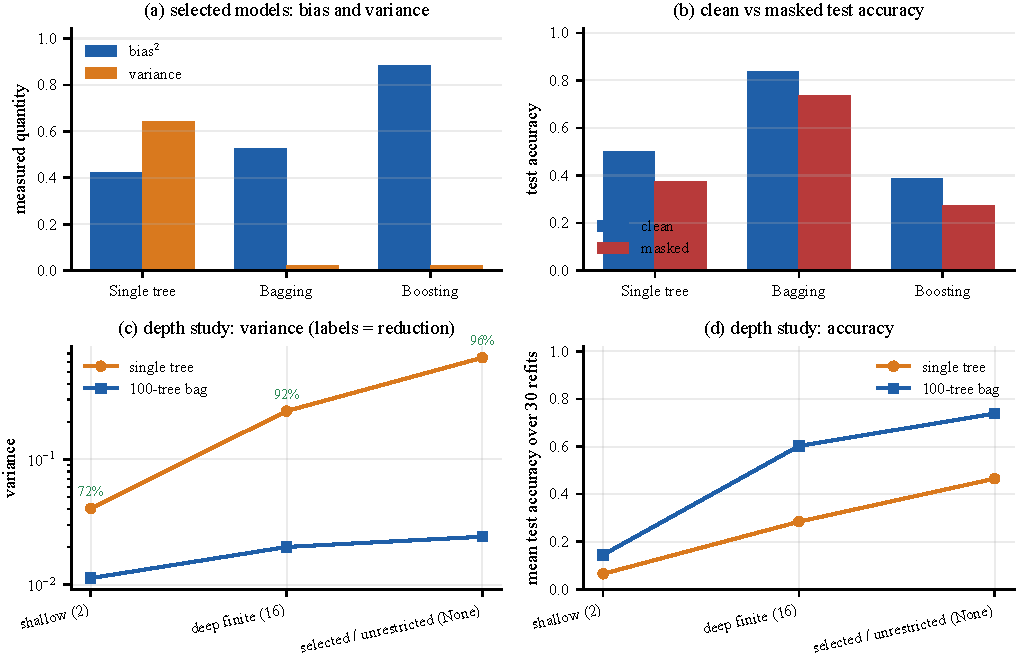
\includegraphics[width=0.86\linewidth]{../figures/fig7_bias_variance.pdf}
\caption{Q3 results.  (a) Measured squared bias and variance for the selected
models over 30 within-identity resamples.  (b) Clean and masked test accuracy.
(c) Variance of the single tree and a 100-tree bag at three depths, with the
percentage reduction printed above each pair.  (d) Mean test accuracy over the
same 30 refits.}
\label{fig:biasvar}
\end{figure*}

\subsection{Depth study}

The selected tree is unrestricted, so ``deeper than selected'' is not defined.
We therefore compare a shallow tree (depth 2), a deep finite tree (depth 16) and
the selected unrestricted tree (depth \texttt{None}), each with a matched
100-tree bag.  Figure~\ref{fig:biasvar}(c,d) gives the
results.

Depth 2 has only \DepthShallowLeaves~leaves (mean occupancy \DepthShallowMeanLeaf, singleton
fraction \DepthShallowSingleton); it underfits, with bias$^2$ \DepthShallowSingleBias,
variance \DepthShallowSingleVar~and accuracy \DepthShallowSingleAcc.  Its bag raises
accuracy to \DepthShallowBagAcc, but the bias stays at \DepthShallowBagBias.  Depth 16 has
\DepthMidLeaves~leaves and variance \DepthMidSingleVar; the bag cuts variance by
\DepthMidVarRed\% and raises accuracy from \DepthMidSingleAcc~to \DepthMidBagAcc.
The unrestricted tree has \DepthDeepLeaves~leaves (mean occupancy
\DepthDeepMeanLeaf), variance \DepthDeepSingleVar~and disagreement \DepthDeepDis; its bag
cuts variance by \DepthDeepVarRed\%, but raises bias from \DepthDeepSingleBias~to
\DepthDeepBagBias, and raises accuracy to \DepthDeepBagAcc.

The largest accuracy gain is at depth \LargestImprovementDepth
(\LargestImprovementGain).  Thus the answer to the assignment's question is
\textbf{\DeepestLargest}: the deepest tree is not necessarily the depth at which
bagging gives the largest accuracy improvement.  The deepest tree is where
bagging removes the most variance---\DepthDeepVarRed\% versus \DepthMidVarRed\% at
depth 16 and \DepthShallowVarRed\% at depth 2---because it has the most leaves and the
largest across-resample variance.  But the extra variance removal is partly
offset by a larger bias increase: bagging raises bias from \DepthDeepSingleBias~to
\DepthDeepBagBias~at the unrestricted depth, compared with \DepthMidSingleBias~to
\DepthMidBagBias~at depth 16.

The disagreement numbers rule out a simple ``more diversity is better''
explanation.  Pairwise disagreement between the 100 bagged trees is highest for
the shallow trees (\DepthShallowDis), lower at depth 16 (\DepthMidDis) and lowest at the
unrestricted depth (\DepthDeepDis).  Deep trees all converge on the same
clean-training partition, so they disagree less with each other, even though
their predictions move most when the training set is resampled.  Disagreement
measures diversity within one ensemble; variance measures sensitivity across
resamples.  Leaf occupancy tells the other half of the story: depth 2 has only
\DepthShallowLeaves~leaves and cannot fit the identities, while the unrestricted tree
has \DepthDeepLeaves~leaves with mean occupancy \DepthDeepMeanLeaf~and the lowest
singleton fraction.  The depth-16 tree has \DepthMidLeaves~leaves, enough to fit
but less extreme than the unrestricted tree, which is why its bias penalty from
bagging is smaller and its accuracy gain is largest.  Variance reduction is
necessary for the gain, but it is not sufficient when the bias penalty also
grows.

Table~\ref{tab:final} answers the stability question directly.  Boosting has
the lowest variance in probability space (\BoostVar, marginally below bagging's
\BagVar), but its refit accuracy is \BoostRefitAcc~$\pm$~\BoostRefitStd, so low
variance does not imply good predictions: its bias dominates.  Bagging has the
smallest accuracy standard deviation (\BagRefitStd) and the best clean and
masked accuracy.  The single tree has the largest absolute clean-to-masked
drop (\TreeCleanDrop, versus \BagCleanDrop~for bagging and \BoostCleanDrop~for
boosting), and it is maximally confident in both conditions.
The lowest-variance model is therefore not the best model; the best model is the
one that balances the two terms, which here is bagging.

\section{Discussion}

\paragraph{Why bagging wins.}  The unrestricted tree has relatively low bias and
high variance~\cite{dietterich2000}: it can represent the training set almost
perfectly, but a different bootstrap sample produces a different set of
axis-aligned splits.  Averaging 200 such trees removes almost all of the
variance (a factor of \BagVarRatio) at the cost of a modest bias increase
(\BagBiasDelta), which is why bagging gains 0.3375 test accuracy over the single
tree and loses only 0.1000 under the mask.  The gain is not free: the bag is 200
times more expensive to fit, and its confidence is lower (mean winning vote
0.3934 clean, 0.2657 masked) because vote fractions are not calibrated
probabilities.

\paragraph{Why boosting struggles.}  SAMME is designed for weak learners that
are slightly better than random.  With 40 classes the random threshold is 0.975,
and a depth-4 tree on 240 faces has weighted error around 0.61, so it is
accepted but weak.  Reweighting then concentrates on a small set of hard faces
(the top ten hold 0.4481 of the weight), which reduces the effective sample size
and makes the next tree even more specialised.  The result is a stable but
biased ensemble: variance is low, bias is high, and 100 rounds do not beat 50.
Boosting would likely benefit from soft class probabilities, more data, or
weak learners with more capacity; those are outside the assignment's frozen
protocol.

\paragraph{Mask behaviour.}  The mask is a best-case test for ensemble diversity
and a worst-case test for any model that relies on the central face region.  A
single bootstrap tree collapses to 0.0250 masked accuracy, the selected tree
drops from 0.5000 to 0.3750, bagging drops from 0.8375 to 0.7375, and boosting
drops from 0.3875 to 0.2750.  The ordering is unchanged, but the mechanisms
differ: bagging retains a small vote lead for the true class, while boosting's
normalised score flips to a different identity.  The mask case is a reminder
that accuracy under a fixed corruption is not a general robustness guarantee.

\paragraph{Limitations.}  The test set has only 80 images, so one image is 1.25
accuracy points; differences of a few points should not be over-interpreted.
All results come from one split and one seed, as required.  The 30 resamples
estimate refit variability but do not turn the single split into a
cross-validation study.  The bias--variance numbers use the Euclidean
probability decomposition and are not directly comparable to zero-one
decompositions in the literature.  Finally, the serial-equivalent timing is a
hardware-independent proxy, not a benchmark.

\section{Conclusion}

Under a frozen, roll-number-seeded 6/2/2 split and raw 4096-pixel inputs,
bagging is the clear winner: 200 bootstrap trees reach 0.9250 validation and
0.8375 clean test accuracy, and 0.7375 with a centred $16\times16$ test block
zeroed.  A single unrestricted tree overfits and reaches 0.5000 test accuracy.
A from-scratch SAMME implementation is correct and stable---its toy round
matches the closed-form weights, and its weighted error falls from 0.8500 to
0.6143---but its hard-vote multiclass decisions remain weak at 0.3875 test
accuracy.  The measured decomposition explains the ranking: bagging cuts
variance relative to a matched tree, especially at unrestricted depth, while
boosting's low variance is offset by high bias.  The repository contains the
saved split, all predictions and histories, the figures, the full run log, and
a one-command reproduction path.

{
\small
\bibliographystyle{ieeenat_fullname}
\bibliography{main}
}

\end{document}
